\documentclass[justified,nobib]{tufte-handout}

\usepackage{Haust2017verkefnablöð}

\title{Tölvunarfræði 1a - vikublað 1}

\hyphenation{mynumber}

\begin{document}

\section{Uppsetning Matlab}
Matlab er aðgengilegt í tölvuverum VR-II, en fyrsta verkefni flestra í Tölvunarfræði 1a er engu að síður að setja upp Matlab.

Matlab er forritunarmál\eng{programming language} og forritunarumhverfi\eng{development environment} gefið út af Mathworks. 

Til að setja upp Matlab á eigin tölvu er farið inn á \href{http://www.mathworks.com/}{vef Mathworks}\footnote{\url{mathworks.com}} og reikningur stofnaður þar með því að nota \emph{HÍ-tölvupóstfang}.

Best er að sækja \href{https://se.mathworks.com/products/matlab/whatsnew.html}{nýjustu útgáfu af Matlab}\footnote{\url{https://se.mathworks.com/products/matlab/whatsnew.html}} nema viðkomandi tölva sé mjög gömul. Ekki sækja prufuútgáfu.

Þegar skrárnar hafa verið sóttar þarf að fylgja uppsetningarleiðbeiningum, sem eru nokkuð mismunandi á milli stýrikerfa.

Uppsetningarforritið mun bjóða upp á að setja upp alls kyns viðbætur við Matlab. Í Tölvunarfræði 1a munum við ekki nota neina þeirra, nóg er að setja upp grunnforritið.

Fólk á eldri vélum og áhugafólk um opinn hugbúnað\eng{open source software} getur litið til GNU Octave\footnote{\url{gnu.org/software/octave/}} sem staðgengil fyrir Matlab.

\begin{figure}
\caption[Niðurhalstengill fyrir Matlab]{Niðurhalstengill fyrir Matlab mun líklega líta nokkurn veginn svona út á síðu Mathworks.}    
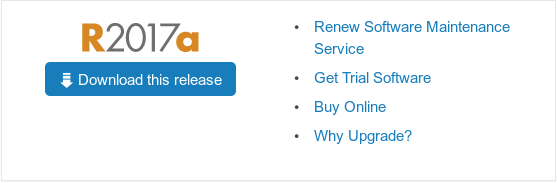
\includegraphics[width=\linewidth]{matlab-download}
\end{figure}

\section{Að opna Matlab}
Þegar Matlab hefur verið sett upp blasa við nokkrir gluggar. Yfirlit yfir helstu hluta viðmótsins má sjá í undirköflum 1.1 og 1.2 í kennslubók. Gluggarnir sem við munum helst nota eru skipanaglugginn \eng{command window} og Matlab-ritillinn \eng{Matlab editor}.

\begin{figure}
\caption[Viðmót Matlab]{Upphafsskjár Matlab mun líta nokkurn veginn svona út. Á þessari mynd sést skipanaglugginn.}
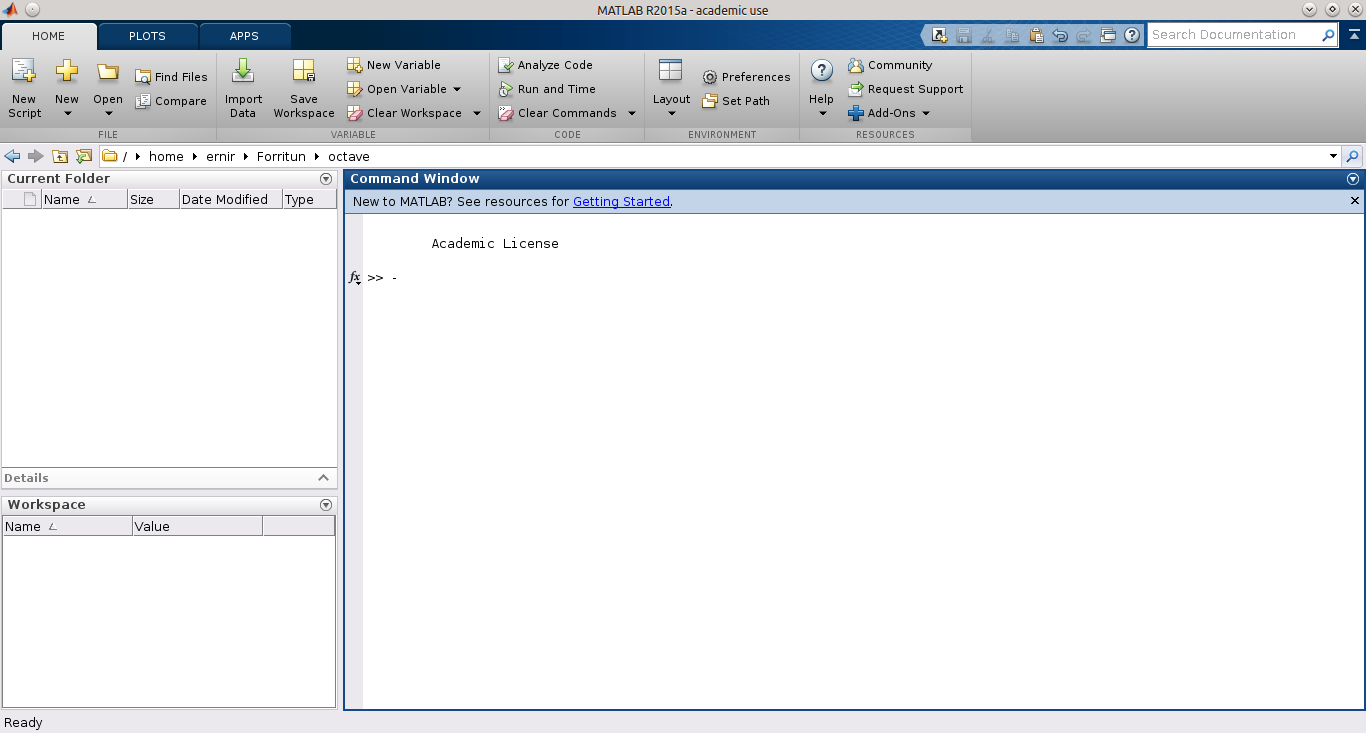
\includegraphics[width=\linewidth]{matlab-gui}
\end{figure}

\subsection{Fyrstu sýnidæmi}
Í fyrsta fyrirlestri verða sýnd sýnidæmi um hvernig hægt er að nota Matlab, m.a. sýnidæmið um hvernig nota má Matlab til að búa til hreyfimynd af pendúl.

Til að búa myndina til eru þekktar jöfnur sem tengjast hreyfingu pendúls notaðar.

Látum $\theta(t)$ tákna útsláttarhorn pendúlsins á tíma $t$, $g$ tákna þyngdarhröðun jarðar og $l$ tákna lengd pendúlsins. Gerum svo ráð fyrir að $\theta$ sé ``lítið'', svo $\sin(\theta) \approx \theta$. 

Þekkt er að hægt er að nálga hreyfingu pendúls með jöfnunni
\[
\frac{d^2\theta}{dt^2} + \frac{g}{l}\theta = 0
\]
sem hefur, með upphafsskilyrðunum $\theta(0) = \theta_0$ og $\frac{d\theta}{dt}(0)= 0$ lausnina
\[
    \theta(t) = \theta_0 \cos\left(\sqrt{\frac{g}{l}}t\right).
\]
En okkar viðfangsefni verður frekar að færa svona jöfnur yfir á snið sem tölva getur skilið. Í Matlab gæti lausnin litið út eins og í forriti \ref{pendulumprogram}.

\begin{example}
\caption{Forrit sem sýnir hreyfimynd af pendúl}
\label{pendulumprogram}
\matlabfile[fontsize=\small]{Code/pendulumexample.m}
\end{example}

\emph{Ekki} er ætlast til að forritskóðinn í sýnidæmi \ref{pendulumprogram} sé skiljanlegur á þessum tímapunkti. Kóðinn er settur fram sem dæmi um að hægt sé að framkvæma útreikninga með Matlab.

\section{Bitar og Bæti}

Ef tölva er vél, þá er hún vél sem færir \emph{bita} á milli ástanda. Öll gögn í tölvum eru geymd sem bitar. 

Líta má á bita sem ``hólf'' af upplýsingum - þar sem einu mögulegu upplýsingarnar eru í hvoru af tveimur ástöndum bitinn er.

Dæmi um einn bita af upplýsingum:
\begin{itemize}
    \item ``Er spenna eða er ekki spenna á þessari rafrás?'' (örgjörvi)
    \item ``Snýr þessi segull norður/suður eða suður/norður?'' (harður diskur)
    \item ``Stutt eða langt?'' (morse-kóði)
\end{itemize}

Hópur af 8 bitum er kallaður bæti. Minnishólfum í tölvum er skipt niður í bæti, ekki er unnið beint með bita.

\subsection{Merking bæta}
Röð af 0 og 1 eins og \texttt{01001011} hefur enga sjálfstæða merkingu. Merking bætanna er ákveðin út frá samhengi.

Bætið \texttt{01001011} gæti verið bókstafurinn 'K' ef við kjósum að túlka það sem ASCII-tölu. Í venjulegu tvíundarkerfi fyrir heiltölur væri það talan 75. Sömuleiðis gæti þetta verið hluti af vélarmálsskipun (mismunandi eftir örgjörvum), kommutölu (sem eru 4 eða 8 bæti) eða stórri mp3, jpeg eða mp4 skrá.

\newthought{Til að geyma tugakerfistölu} sem tvíundarkerfistölu\eng{binary number} er venjulegt að láta bitann í sæti $i$ tákna margfeldi við töluna $2^i$. Útkomur margfaldananna eru svo lagðar saman. Dæmi:
\marginnote{Talan \emph{01001011} er með 0 fremst. Þetta er oft gert þegar tvíundartölur eru skrifaðar, svo að fjöldi bita í tölunni sé margfeldi af 8. Reyndar kemur fremsti bitinn líka við sögu þegar tákna á neikvæðar tölur.}
\begin{align*}
    1 		&=  2^0  	= 1\\
    101		&=  2^2 + 2^0  =  4 + 1  =  5\\
    01001011	&=  2^6 + 2^3 + 2^1 + 2^0  =  64 + 8 + 2 + 1 = 75
\end{align*}

Tvíundartölur eru tölur, svo þær má leggja saman: 
\begin{align*}
    00000001 + 00000010 &= 00000011\\
    2^0 + 2^1 &= 3
\end{align*}

Stærsta tvíundartala sem hægt er að tákna með einu bæti hlýtur þá að vera $11111111$, sem er talan $128+64+32+16+8+4+2+1$  $=  255$. Tilraunir til að vinna með stærri tölur en geymslusvæðið býður upp á veldur svokölluðu reikningsyfirflæði\eng{arithmetic overflow}.

Til að tákna neikvæðar heiltölur er algengast að nota tvíandhverfu\eng{two's complement}. Til að reikna út tvíandhverfu tvíundartölu er hægt að snúa öllum bitunum við og leggja 1 við.

\begin{margintable}
\caption{Hægt er að túlka sömu bitarunu á mismunandi vegu.}
\begin{tabular}{lrr}
\toprule
Bitar&Formerkislaust&Tvíandhverfa\\
\midrule
\texttt{01111111}&127&127\\
\texttt{01111110}&126&126\\
\texttt{00000010}&2&2\\
\texttt{00000001}&1&1\\
\texttt{00000000}&0&0\\
\texttt{11111111}&255&-1\\
\texttt{11111110}&254&-2\\
\texttt{10000010}&130&-126\\
\texttt{10000001}&129&-127\\
\texttt{10000000}&128&-128\\
\bottomrule
\end{tabular}
\end{margintable}

Útkoman er sú að ef að við lesum ákveðna runu af bitum sem heiltölu sem getur verið neikvæð\eng{signed integer}, þá táknar runan neikvæða tölu ef bitinn sem lengst er til vinstri er 1. Þetta gerir það að verkum að það bil jákvæðra talna sem kemst fyrir í minnishólfinu minnkar.

\section{Breytur}
Við könnumst við breytur\eng{variables} eins og $x$ og $y$ úr stærðfræði. Í forritun koma fyrir breytur sem hafa að sumu leyti hliðstæða eiginleika.

Gefum okkur að við höfum aðgang að minni í tölvu, þar sem upplýsingar sem samanstanda af bætum eru geymdar. Breyta í forriti er afmarkað minnishólf sem inniheldur gildi.

Til að geta vísað í minnishólfið gefum við því nafn, svokallað breytuheiti\eng{variable name}.

Hver breyta er af ákveðinni gagnagerð\eng{data type, class. Gagnagerð er einnig þekkt sem ``tag'' á íslensku.} sem segir til um hve stórt minnisvæðið sem breytan tekur til er og hvernig skal túlka það.

\newthought{Til að búa til breytu í Matlab} er nafn hennar fyrst skrifað, svo jafnt og merki, svo gildið sem breytan skal fá. Í skipanaglugganum gæti þetta litið svona út:

\begin{example}
\caption{Breytan \texttt{mynumber} búin til. Í sýnidæmum í þessu námskeiði munu tveir goggar (>>) gefa til kynna að um skipun sem keyra megi í skipanaglugganum sé að ræða.}
\begin{minted}[frame=lines]{matlab}
>> mynumber = 6
mynumber =  
     6
\end{minted}
\end{example}

Merking skipunarinnar í efstu línunni er ``settu gildið $6$ í breytuna \texttt{mynumber}''. Matlab svarar með gildi nýju breytunnar.

Sé semíkomma sett á eftir skipuninni svarar Matlab ekki. Þetta er æskilegt þegar forrit eru skrifuð.

Workspace-glugginn í Matlab viðmótinu sýnir ýmsar upplýsingar um skilgreindar breytur. Hægri-smella má á dálkana til að sýna fleiri.
\begin{marginfigure}
\caption{Mögulegt útlit workspace-gluggans}    
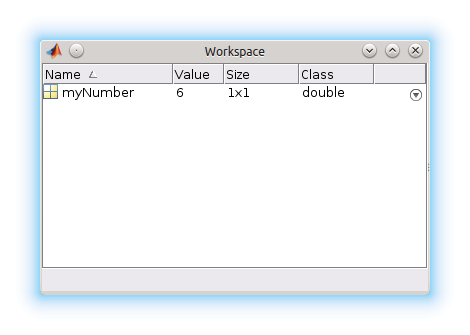
\includegraphics[width=\linewidth]{Pics/workspace-window}
\end{marginfigure}

\newthought{Breytan ans} er sérstök í Matlab. Henni er sjálfkrafa gefið gildi þegar reiknisetning er framkvæmd án þess önnur breyta sé tiltekin til að geyma niðurstöðuna.
\begin{example}
\caption{Breytan \texttt{ans} fær gildi}
\begin{minted}[frame=lines]{matlab}
>> 2+3
ans = 
     5
\end{minted}
\end{example}

Breytur geymast á milli skipana, svo hægt er að nota þær áfram.

\begin{example}
\caption{Breytur notaðar aftur eftir að þær hafa verið skilgreindar.}
\begin{minted}[frame=lines]{matlab}
>> x = 1;
>> y = 2;
>> x + y
ans =
     3
\end{minted}
\end{example}

Breyta helst skilgreind þar til henni er eytt eða þar til við förum út úr sviði \eng{scope} breytunnar (meira síðar).

\subsection{Breytuheiti}

Breytur í forritum verða oft mjög margar, mikilvægt er að gefa þeim lýsandi heiti. T.d. merking skipunarinnar 
\begin{center}
    \texttt{force = mass * acceleration}
\end{center} 
skýrari en merking skipunarinnar \texttt{z = x * y}. Tölvur eiga ekki í neinum vandræðum með að lesa löng orð, svo við val á breytuheitum ætti helst að hafa í huga hversu merkingarbær þau eru fyrir mennska lesendur.

Ekki eru öll orð lögleg breytuheiti í Matlab. Til dæmis mega breytur í Matlab ekki hafa nöfn sem byrja á tölustaf eða nöfn sem innihalda íslenska stafi. Lesa má um lögleg breytuheiti og skipanir sem tengjast breytum í kafla 1.3.2 í kennslubók.

\subsection{Gagnagerðir}
Allar breytur hafa gagnagerð (tag). Matlab ákvarðar gagnagerðina sjálfkrafa út frá gildinu sem breytunni er gefið.
Helstu tög eru:
\begin{itemize}
\item Kommutölur. Þær má sem má setja fram með tögunum \texttt{single} og \texttt{double}. Sjálfgefna tagið fyrir tölur í Matlab er \texttt{double}. Tögin \texttt{single} og \texttt{double} eru fleytitölutög\eng{floating point types}.
\item Heiltölur\eng{integers}. Heiltölur hafa tögin \texttt{int8}, \texttt{int16}, \texttt{int32} og \texttt{int64}, þar sem talan táknar fjölda bita sem notaðir eru til að geyma töluna. 
\item Bókstafir \eng{characters} eru geymdir í breytum af gerðinni \texttt{char}. Dæmi um slíkar breytur eru \texttt{'a'} og \texttt{'halló heimur'}.
\item Rökgildi\eng{logical values, boolean values} hafa gerðina \texttt{logical}. Slíkar breytur hafa bara tvö möguleg gildi: \texttt{true} og \texttt{false}, sem samsvara tölunum 1 og 0.
\end{itemize}
Við munum sjá fleiri tög eftir því sem á líður námskeiðið.

\section{Útreikningar með Matlab}

\section{Textaframsetning með LaTeX}
Raungreinafólk notar oft textaframsetningarkerfið LaTeX (\LaTeX) til að koma skýrslum, greinum og verkefnum frá sér á staðlaðan og faglegan hátt.

LaTeX er ólíkt ritvinnslukerfum eins og Microsoft Word og LibreOffice að því leyti að í LaTeX er ekki unnið beint með skjalið eins og það mun líta út við útgáfu, heldur með hrátt textaskjal sem síðar er þýtt\eng{compiled} yfir í birtingarhæft skjal. Vinnsla með LaTeX er þannig nokkurs konar forritun. Við látum tölvunni í té upplýsingar um hvernig skjalið skal líta út og tölvan sér um að vinna úr því.

Þetta fyrirkomulag hefur nokkrar afleiðingar, sumar óheppilegar. Nauðsynlegt er að þekkja helstu LaTeX skipanirnar til að geta komið efni frá sér. Erfitt getur verið að ná fram ákveðnu útliti á lokaskjalinu.

Meðal kostanna er að ekki þarf að hugsa um útlitsstillingar, útkoman er stöðluð. Hægt er að einbeita sér að uppbyggingu textans.
LaTeX er með gríðarsterkan stuðning fyrir framsetningu á stærðfræðitáknum og utanumhald á heimildaskrám.

\begin{example}
\caption{LaTeX kóði}
\begin{minted}[frame=lines]{latex}
\[\int_{0}^{2\pi} x^2 dx\]
\end{minted}
\end{example}

\subsection{Að læra LaTeX}
Við munum ekki fara djúpt í virkni LaTeX í þessu námskeiði, enda er það ekki nauðsynlegt til að koma frá sér skjali.

Lengi vel var eitt erfiðasta skrefið við að læra LaTeX það að setja upp LaTeX-þýðanda. Í dag er hægt að þýða LaTeX skrár á netinu í gegnum þjónustur eins og \href{https://www.overleaf.com/}{Overleaf}\footnote{\href{https://www.overleaf.com/}{overleaf.com}}, svo þjáningin ætti að vera minni í upphafi.

Sjá \href{https://www.overleaf.com/read/hrhjkyvxdhrf}{sýnidæmi}\footnote{\href{https://www.overleaf.com/read/hrhjkyvxdhrf}{overleaf.com/read/hrhjkyvxdhrf}} um skjal með flestum þeim skipunum sem á þarf að halda.

\end{document}